% %%%%%%%%%%%%%%%%%%%%%%%%%%%%%%%%%%%%%%%%%%%%%%%%%%%%%%%%%%%%%%%%%%%%%%%%%%%%%%%%%
To have correct input of fresh water is important to understand the circulation in the surface layer of a fjord system. Two of the major rivers in Norway drain into the FjordOs model domain, Glomma$^1$ and Drammenselva$^1$, with annual mean discharge of 729 and 317 m$^3$/s, respectivly \citep{milli:etal:2011}. 
In a textbook example of a fjord, the river outlet is located at the fjord head, and it is often found what is called an estuarine circulation with a fresh surface layer flowing from the river outlet and toward the sea. In contrast to this the Glomma outlet is situated in the outer part of the Oslofjord,
and the outlet of Drammenselva is situated in the middle part of the fjord system. As a result of this the estuarine circulation in the Oslofjord can deviate considerably from the classical textbook example. 
To add to the complexity several small and large rivers and streams is also found in the area, and a total of 37 rivers are included in the model setup. The discharge from the two largest rivers are divided and released into different receiving model grids cells (see Table \ref{tab:riv1}\footnote{In this report it is chosen to use Norwegian river names in which ``elv'' or ``vassdrag'', means ``river'' or ``water course''.}). As can be seen from Fig. \ref{fig:riv1}, where all the rivers in the area are shown, many more rivers could have been included in the model. This could be a task for further development of the model.
%% %%%%%%%%%%%%%%%%%%%%%%%%%% Figure 1 Oversiktskart %%%%%%%%%%%%%%%%%%%%%%%%%%%%
\begin{figure}[t]
 \setlength{\unitlength}{1.0cm}
 \begin{center}
  \begin{pspicture}(0,0)(14,20)
% Include graphs
   \rput[b](7,0){\includegraphics[height=20cm]{Elver_Oslofjorden_v3.eps}}
%   \includegraphics[height=15cm]{images/Elver_Oslofjorden_v3.eps}
  \end{pspicture}
% Figure caption is below the figure
  \caption{Map showing all the rivers flowing into the Oslofjord (NVE Elvenett).
  Some of the larger rivers are marked with a thicker blue line.
  Stations with water discharge measurements are shown with green dots.
  River outlets included in the FjordOs model is shown with red dots.}   
  \label{fig:riv1}      
 \end{center}
\end{figure}
%


%\input{river_table1.tex}

The rivers are sources of nutrients, organic matter, bacteria, particles and contaminants, as well as freshwater. Several of these parameters are monitored in a national monitoring program (Riverine Inputs and direct Discharges - RID, \cite{skarb:etal:2011}). An overview of the RID stations and what parameters that are measured are shown in Table \ref{tab:riv2}. If the FjordOs CL is used to model dispersion of any of these parameters, information from the RID program can be included in the river forcing.
%\input{river_table2.tex}

The catchment area draining into the fjord within the FjordOs model domain, contains 15 of the main catchment areas (MCA) in Norway. Let $A_i$ be the area for each of the MCAs $i$. Each of the MCAs contain one or more rivers, each representing a portion of the MCA, $a_j$, where $J_i$ is the number of rivers within the MCA. 
\be
  \label{eq:riv01}
   A_i = \sum_{j=1}^{J_i} a_j.
\ee
Let $Q_i$ be the freshwater discharge from the entire MCA into the sea, and let $q_j$ be the water discharge for the individual river. We assume that the river discharge for the individual rivers are entirely determined by the size of the portion of the MCA that drain into this river. Then we can write 
\be
 \label{eq:riv02}
  q_j = \frac{a_j}{A_i} Q_i.
\ee
A consequence of this assumption is that the total discharge from a MCA can be determined by any one of the rivers within it 
\be
 \label{eq:riv03}
 Q_i = \frac{A_i}{a_j} q_j.
\ee

In this project several sources of information about river discharge is considered.

\begin{itemize}
\item Model data for each MCA.
\item Observations from the NVE website. 
\item Observations from other sources (Oslo municipality, glb.no).
\end{itemize}

The entire country is set up with a catchment area model called HBV \citep{beldr:etal:2003}. This modelling task is performed once a year, giving a hindcast of the discharge of every MCA from 1962 up till the previous year, with daily temporal resolution. This dataset is used for hindcast runs with the Norkyst800 model \citep{albre:etal:2011}. Equation (\ref{eq:riv02}) and values from Table \ref{tab:riv1} give the required information to estimate the discharge of each individual river in the FjordOs model.

In some of the rivers observations are available in near real time. At seven stations shown in Table \ref{tab:riv3} and plottet in Fig. \ref{fig:riv1}, observations can be downloaded in near real time from the NVE website (www2.nve.no/h/hd/plotreal/Q/index.html). The seven stations corresponds to river no. 1 (Haldenvassdraget), no. 2-7 (Glomma), no. 13 (Mosseelva), no. 21 (Akerselva), no. 25 (Sandvikselva), 
no. 34-38 (Drammenselva) and no. 46 (Nummedalsl{\aa}gen).

Observations are also available from other sources. The water and sewerage unit in the Oslo municipality operates several water discharge stations in the Oslo area. Particularily observations from Lysakerelva in MCA no. 7 is of intrest to the FjordOs model, but this is not considered in this report. Glommens og Laagens Brukseierforening (glb.no) have observations in Glomma at the station Sarpsfoss close to the river outlet. Observations from this station is at the time of writing available up til October 28$^{th}$ 2015, and therefore it is of interest to check the correlation between the NVE stations and Sarpsborg. The correlation is shown in Table \ref{tab:riv3}, and the river discharge in Mosselva (MCA no. 3), Akerselva (MCA no. 6) and Drammenselva (MCA no. 12) can be estimated with fairly good accuracy based only on measurments at Sarpsfoss. In the other rivers the correlation is poor. This is because the shape of flood episodes are differnt in these rivers (see Fig. \ref{fig:riv3}).

By the use og eq. (\ref{eq:riv03}) the discharge from MCA, $Q_i$, with $i$=1, 2, 3, 6, 8, 12, and 15 can be calculated from the seven NVE stations. For MCA no. 2, the NVE stations is situaded far up in the river. In this case a correction factor is estimated based on least square fit between observations at R{\aa}n{\aa}sfoss, $q_2$ and Sarpsfoss, $q_{sarpsfoss}$.
\be
 \label{eq:riv04}
 q_{sarpsfoss} = 1.123 \cdot q_{2} 
\ee
Eq. (\ref{eq:riv04}) gives an estimate of the river discharge in Glomma with an RMS error of about 100 m$^3$/s.
%\input{river_table3.tex}
%% %%%%%%%%%%%%%%%%%%%%%%%%%% Figure 1 Oversiktskart %%%%%%%%%%%%%%%%%%%%%%%%%%%%
\begin{figure}[t]
 \setlength{\unitlength}{1.0cm}
 \begin{center}
  \begin{pspicture}(0,0)(14,20)
% Include graphs
   \rput[b](7,0){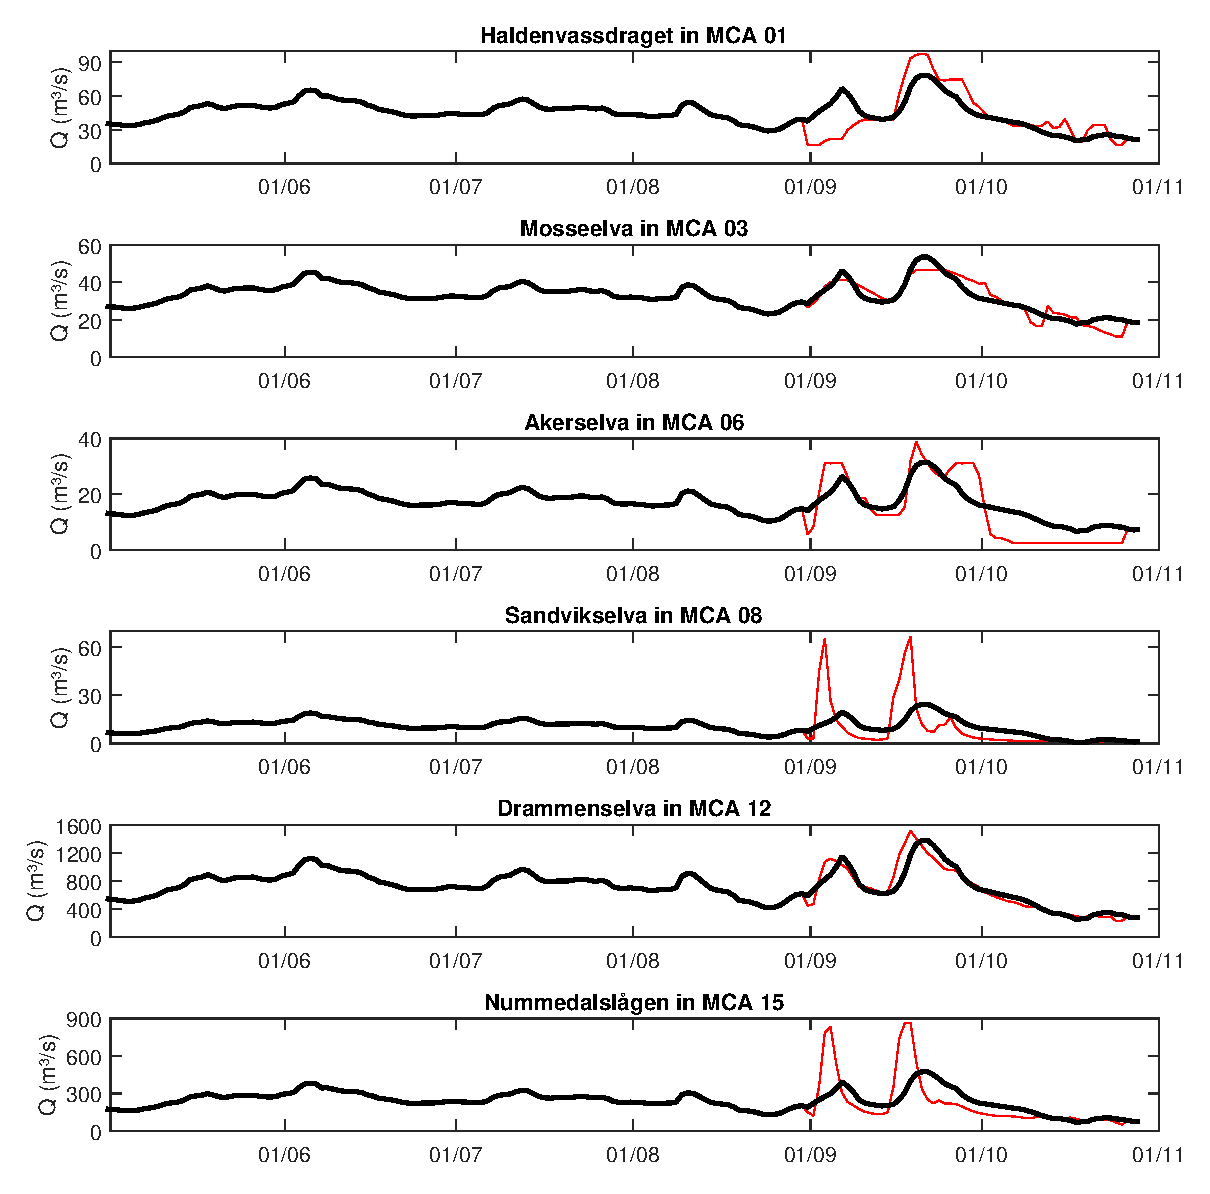
\includegraphics[height=20cm]{images/Q_obs_vs_1river_estimate.eps}}
%   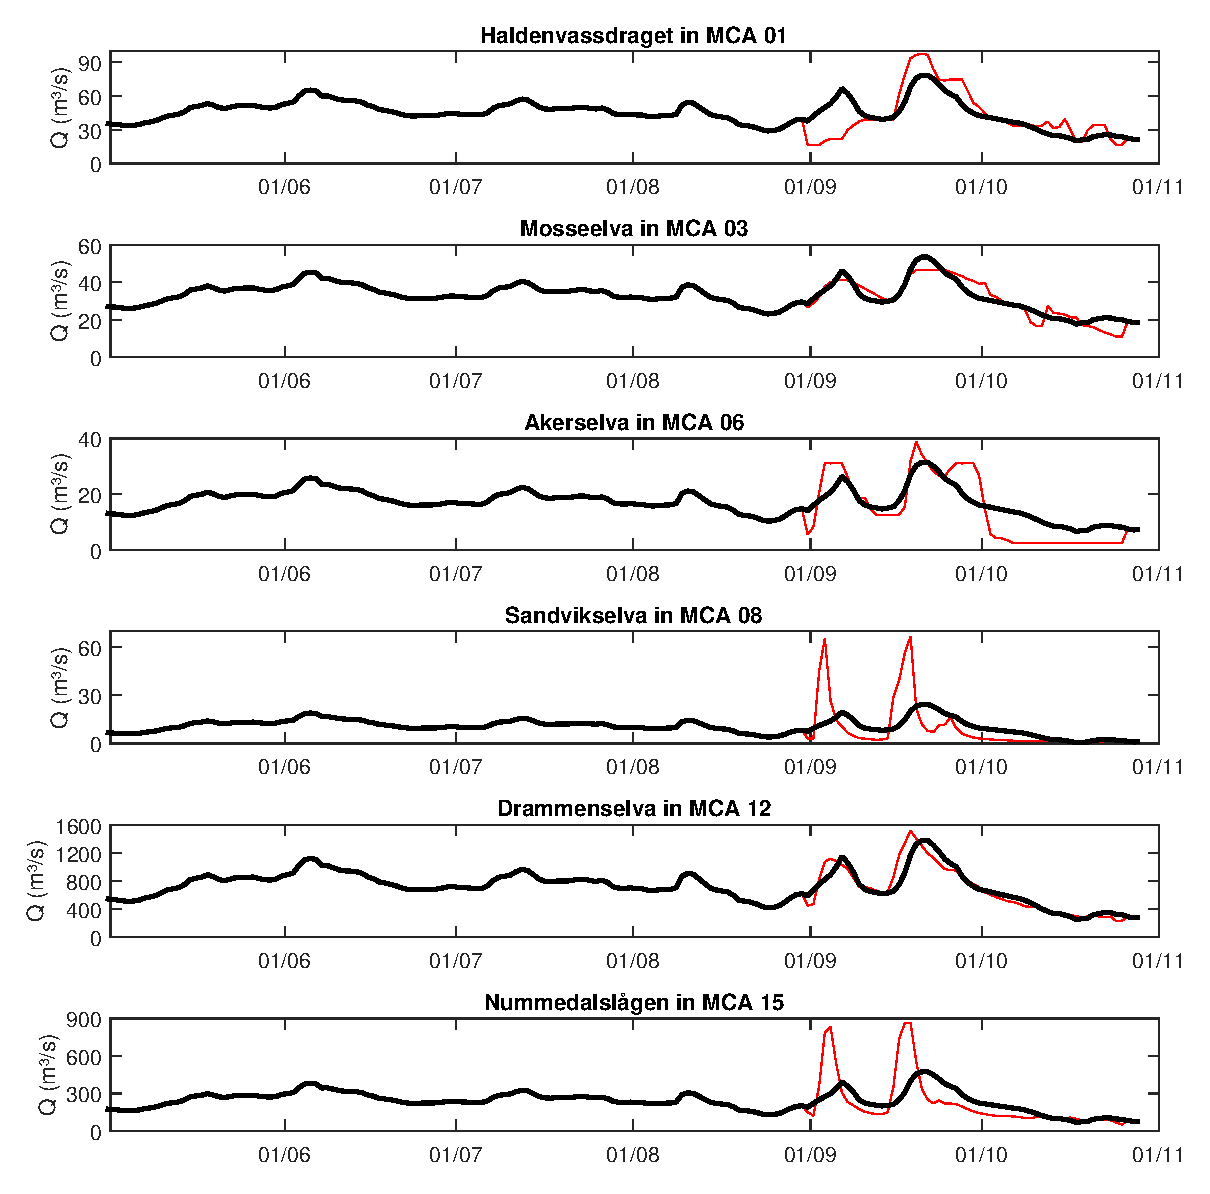
\includegraphics[height=15cm]{images/Q_obs_vs_1river_estimate.eps}
  \end{pspicture}
% Figure caption is below the figure
  \caption{Comparison between river discharges estimated based on observations from
  Sarpsfoss (black line), and observations (red line), in six rivers.
  }   \label{fig:riv3}      
 \end{center}
\end{figure}
%



For some of the 15 MCAs in the model domain, no observations are available ($i=$ 4, 5, 7, 9, 10, 11, 13, 14). It is therefore attempted to find relationships between the discharge of the observed and the unobserved MCAs based on model data. MCA no. 2 (Glomma), 3 (Mosseelva), 8 (Sandvikselva) and 15 (Nummedalsl{\aa}en) was used. An auxilirary parameter was calculated that was the sum of the river discharge of all combinations of the four rivers. A least mean square fit was performed between this new parameter and the discharge for the MCA in question 
\be
 \label{eq:riv05}
 Q_i = \alpha_i \left(f_i^2 Q_2 + f_i^3 Q_3 + f_i^8 Q_8 +f_i^{15} Q_{15}\right) + \beta_i 
\ee
The result of this analysis is shown in Table \ref{tab:riv4}. It is a little surprising that the discharge from MCA no. 2 and 15 did not improve the estimate of the discharge from the other MCAs.   
%\input{river_table4.tex}

 
 
 
